\section{Lexer and parser generation}\label{sec:lexerandparsergen}
This section briefly covers how the lexer and parser for Arc has been implemented, and what alternatives could have been used.

The lexer, also called a lexical analyzer or scanner, takes a character stream and turns it into tokens. Tokens are a representation of something in a language, such as a num in Arc would be a token, that represents numbers. The lexer recognizes and can discard characters of the character stream, so that the parser can ignore them. For example whitespaces, that the parser does not need to concern itself with. If the lexer did not discard these, the parser would constantly have to check for them. These tokens are then passed to the parser, that makes syntatic sense of them. It compares the tokens and their structure to the grammar of the specific language.\cite{Parr2014}

For Arc, \gls{antlr} has been used, for creating the grammer and also to generate both the lexer and parser. From writing the grammar, is was possible for \gls{antlr} to generate the lexer, parser and more.\cite{Parr2014} This made \gls{antlr} highly effective for designing Arc, as small changes to the grammar could easily be made, without having to re-create the lexer and parser everytime. Instead only the grammar had to be changed, and \gls{antlr} would generate a new lexer and parser, based on the new grammar.

The grammar was made in a file called 'arcv2.g4' which is an \gls{antlr} file, that \gls{antlr} recognizes and also the lexical rule were made in a file called 'lexerRules.g4'. With these files, \gls{antlr} could generate all needed files for the parser, the lexical analyzer, and other supporting files.


\begin{figure}[htb!]
    \begin{center}
        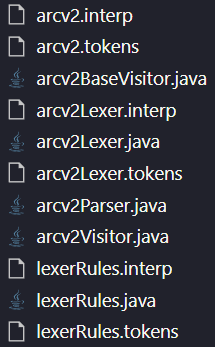
\includegraphics[width=0.25\textwidth]{figures/lexerAndParserFiles.png}
        \caption{Files generated for Arcs parser and lexical analyzer}
        \label{fig:lexerandparserfiles}
    \end{center}
\end{figure}


Figure \ref{fig:lexerandparserfiles} shows the files that \gls{antlr} generates for the lexer, parser and visitor, from the grammar rules and lexical rules. The file 'arcv2Parser.java' is the parser, 'arcv2lexer.java' is the lexical analyzer, 'arcv2Visitor.java' and 'arcv2BaseVisitor.java' are the visitor methods and the interface for the visitor methods. There will not be gone into depth of the contents of these files, as they are not meant to be understood clearly of users, but rather only for the functions in these files to be used. \question{Kan vi sige det sådan her?}


\begin{listing}[htb!]
    \begin{minted}{java}
        CharStream input = CharStreams.fromFileName("src/astTestFile.txt");
        arcv2Lexer lexer = new arcv2Lexer(input);
        CommonTokenStream tokens = new CommonTokenStream(lexer);
        arcv2Parser parser = new arcv2Parser(tokens);
        ParseTree tree = parser.start();
        //EvalVisitor eval = new EvalVisitor();
    \end{minted}
    \caption{An example of how the parser and lexer is used}
    \label{lst:parserandlexerexample}
\end{listing}


Listing \ref{lst:parserandlexerexample} shows how the parser, lexer and visitor are used in practise. Line 1 creates an input based on a file, this input is a stream of characters, that can the be used for the lexer seen on line 2. Line 2 then creates a variable 'lexer', that uses Arcs lexer on input, this variable is then used on line 3 as a paramater of the function CommonTokenStream, to create the tokens. These tokens are then used on line 4 in the parser function arcv2Parser, to create the variable 'parser'. This variable is used on line 5, to create the \gls{cst}, with the .start method, to create the variable 'tree'. \question{Is this descriptive enough of what happens and is it correct? And do we want to include line 6 as it is the visitor}


Another option to this could have been, writing out both the parser and lexer by hand, this could be very educational, as creating our own parser and lexer, would give in-depth knowledge of how they each work. But this would increase the time needed to create Arc considerably as, as mentioned previously, any minor change made in the grammar, would also mean going through the lexer and parser to fix them accordingly. This could lead to time wasted, which is a limiting factor for this project. Therefore it was decided to use the obviouse solution, to use the tools that readily avaliable. For this reason in particular, using \gls{antlr} to generate the lexer and parser for us, was the obviouse choice.

